\clearpage
\title{Finding root of nonlinear equation using False Position Method.}
\author{}
\date{}
\maketitle

\section*{Introduction}
\subsection*{False Position Method}
False position method is based on the fact that if $f(x)$ is real and continuous function, and for two initial guesses $a$ and $b$ brackets the root such that: $f(a)\times f(b) < 0$ then there exists at least one root between $a$ and $b$.\\\\
If $a$ and $b$ are two guesses then we compute new approximated root as:
\[c = a - \frac{f(a)\times (b-a)}{f(b) - f(a)}\]
Now we have following three different cases:
\begin{itemize}
    \item If $f(c)=0$ then the root is c.
    \item If $f(a)\times f(b)< 0$ then root lies between $a$ and $c$.
    \item If $f(a)\times f(c)> 0$ then root lies between $b$ and $c$.
\end{itemize}
And then the process is repeated until we find the root within desired accuracy.\cite{falsePos}


\section*{Tools Used}
\begin{itemize}
    \item MATLAB R2021a - for writing and running code.
    \item MacTeX -\LaTeX  compiler.
    \item VS Code with \LaTeX workshop extension as a text editor.
\end{itemize}

\section*{Process}

\subsection*{Code for False Position:}
\begin{minted}[breaklines, linenos]{matlab}
% Clearing Screen
clc
% Setting x as symbolic variable
syms x;

% Input Section
eqn = input('Enter non-linear equations: ');
a = input('Enter first guess: ');
b = input('Enter second guess: ');
e = input('Tolerable error: ');

% Finding Functional Value
fa = eval(subs(eqn,x,a));
fb = eval(subs(eqn,x,b));

% Implementing False Position Method
if fa*fb > 0 
    disp('Given initial values do not bracket the root.');
else
    c = a - (a-b) * fa/(fa-fb);
    fc = eval(subs(eqn,x,c));
    fprintf('\n\na\t\t\tb\t\t\tc\t\t\tf(c)\n');
    while abs(fc)>e
        fprintf('%f\t%f\t%f\t%f\n',a,b,c,fc);
        if fa*fc< 0
            b =c;
            fb = eval(subs(eqn,x,b));
        else
            a =c;
            fa = eval(subs(eqn,x,a));
        end
        c = a - (a-b) * fa/(fa-fb);
        fc = eval(subs(eqn,x,c));
    end
    fprintf('\nRoot is: %f\n', c);
end
\end{minted}

\subsection*{Output}
\begin{center}
    \centering
    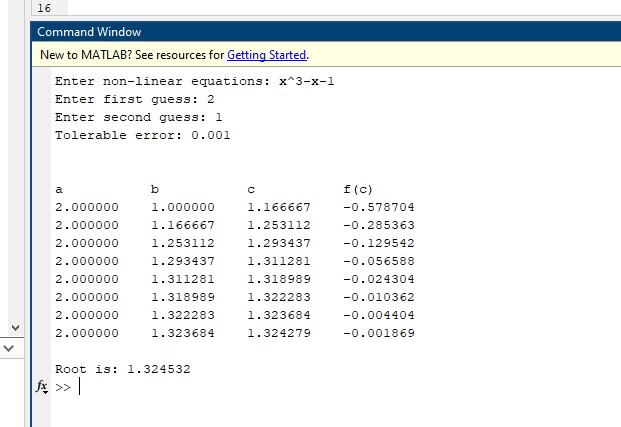
\includegraphics[width = .9\textwidth]{false.jpeg}
    \captionof{figure}{Flase Position method}
\end{center}




